\documentclass[main.tex]{subfiles}
\begin{document}
\session{02}{19-11-2026}

New in this session:
\begin{itemize}[nosep]
  \item race conditions
  \item atomic functions: \texttt{atomicAdd}, \texttt{atomicSub}, \texttt{atomicMin}, \texttt{atomicMax}, \texttt{atomicExch}, \texttt{atomicCAS}
  \item reduction and \texttt{\_\_syncthreads()}
  \item \texttt{\_\_shared\_\_} memory
  \item timing with CUDA events and \texttt{std::chrono}, \texttt{cudaMemset}
  \item locks and \texttt{\_\_threadfence()}
\end{itemize}

%=====================================================================
\section{Reading}

CUDA Programming Guide:
\begin{itemize}[nosep]
  \item Atomic functions:\\
    \url{https://docs.nvidia.com/cuda/cuda-programming-guide/05-appendices/cpp-language-extensions.html#atomicadd}
    \item Maximum intensity projection (Wikipedia):\\ \url{https://en.wikipedia.org/wiki/Maximum_intensity_projection}
\end{itemize}

%=====================================================================
\section{Race conditions}
\label{sec:race}

Many threads often have to combine their results into one value: a sum, a maximum, a count.
If they all update the same memory location, updates get lost.

\subsection{One increment is three operations}

Let \texttt{int *x} point to an integer in global memory. \texttt{(*x)++} is executed in three steps:
\begin{enumerate}[nosep]
  \item read the value at \texttt{*x} into a register;
  \item add 1 to the value in the register;
  \item write the result back to \texttt{*x}.
\end{enumerate}

The addition happens in the GPU core (SM), not in memory: the value sits in a register and an integer unit (ALU) adds 1.
Memory can only be read and written, it cannot add. That is why the value travels memory $\rightarrow$ register $\rightarrow$ memory.

\begin{figure}[H]
\centering
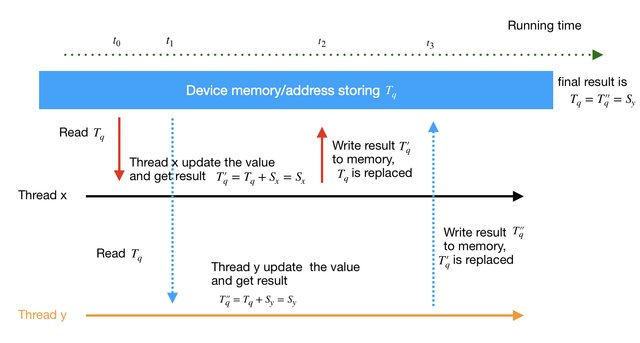
\includegraphics[width=0.72\linewidth, frame]{figures/session_2_figures/race.jpg}
\caption{Race condition: threads x and y both add to the value $T_q$ in memory, which starts at 0.}
\end{figure}

Thread x reads $T_q$ and computes $T_q' = T_q + S_x$ in its register.
Before x has written its result, thread y also reads $T_q$, which still holds the old value, and computes $T_q'' = T_q + S_y$.
x writes $T_q'$, then y writes $T_q''$ and overwrites it.
The final result is $S_y$ instead of $S_x + S_y$: the addition of x is lost.
For a correct result, y may only read after x has written.

\paragraph{Race condition.}
A hazard where the result of a program depends on the timing of events that cannot be controlled, such as the execution order of threads.
It arises when threads do not only work on their own data, but write to a shared location.

Two ways to fix it follow:
\begin{itemize}[nosep]
  \item brute force: atomic operations (Section~\ref{sec:atomics}) and locks force the threads to take turns;
  \item reduction: restructure the computation so that threads no longer write to the same location.
\end{itemize}

\subsection{09\_race\_condition.cu}
\begin{lstlisting}[language=CUDA]
// description: 1,000,000 threads each add one element of an array (all 1) to the same int total. Print the expected and the obtained sum, and the time of the kernel.

#include <cstdio>

#define N 1000000

// total is a pointer to ONE int (not an array): the shared result. *total means "the int that total points to".
// Every thread adds its own element to that one int.
// *total += a[i] is read + add + write. A thread that reads total before another thread has written it computes with an old value, and the writes overwrite each other: increments get lost.
__global__ void sum(const int* a, int* total, int n) {
    int i = blockIdx.x * blockDim.x + threadIdx.x;
    if (i < n) *total += a[i];
}

int main() {
    int *a, *total;
    cudaMallocManaged(&a, N * sizeof(int));
    cudaMallocManaged(&total, sizeof(int));

    // every element is 1, so the correct sum is N
    for (int i = 0; i < N; i++) a[i] = 1;

    // 3907 blocks of 256 threads, one thread per element
    int threads = 256;
    int blocks = (N + threads - 1) / threads;

    // Warm-up: the first launch also includes one-time costs (initialization, moving the managed memory to the GPU).
    // Launch once before timing so you measure the kernel itself. Its result is thrown away.
    sum<<<blocks, threads>>>(a, total, N);

    // cudaMemset(pointer, byte value, number of bytes): sets memory to a value, ON THE GPU.
    // Not *total = 0: a CPU write moves the managed memory back to the CPU, and the timed kernel would first have to move it back to the GPU.
    cudaMemset(total, 0, sizeof(int));

    // CUDA events: timestamps recorded by the GPU itself, in order with the kernels.
    // A CPU timer does not work here: the launch is asynchronous, so a CPU timer would only measure how long it takes to START the kernel.
    // Order: cudaEventRecord(start) -> launch -> cudaEventRecord(stop) -> cudaEventSynchronize(stop): wait until the GPU has reached stop
    // cudaEventElapsedTime: the time between the two events, in milliseconds.
    cudaEvent_t start, stop;
    cudaEventCreate(&start);
    cudaEventCreate(&stop);

    cudaEventRecord(start);
    sum<<<blocks, threads>>>(a, total, N);
    cudaEventRecord(stop);
    cudaEventSynchronize(stop);

    float ms;
    cudaEventElapsedTime(&ms, start, stop);

    printf("expected %d, got %d, in %.3f ms\n", N, *total, ms);

    cudaEventDestroy(start);
    cudaEventDestroy(stop);
    cudaFree(a);
    cudaFree(total);
}

// Output (the sum is lower than 1000000 and changes from run to run; the time depends on the machine):
// expected 1000000, got 88, in 10 ms
//
// The result depends on the timing of the threads: a race condition.
// The 32 threads of a warp execute the read together, so they all read the same old value of *total.
\end{lstlisting}

%=====================================================================
\section{Fix 1: atomic operations}
\label{sec:atomics}

One way to avoid the race: lock the value while a thread updates it. Thread x reserves the lock, does its read + add + write and releases the lock; thread y waits until then.

\begin{figure}[H]
\centering
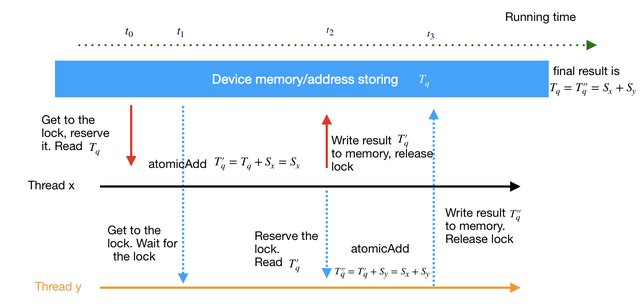
\includegraphics[width=0.72\linewidth, frame]{figures/session_2_figures/atomic.jpg}
\caption{Resource locking: thread y waits until thread x has released the lock on $T_q$. The final result is $S_x + S_y$.}
\end{figure}

An atomic operation such as \texttt{atomicAdd} is this, done by the hardware for one read + modify + write: no other thread can access the address in between.
Atomics on the same address are executed one after another, so the result is always correct, but those threads no longer work in parallel.
How much time that costs depends on the GPU: the compiler and newer hardware combine some atomics on the same address. 09 and 10 measure it.

\subsection{10\_atomic\_add.cu}
\begin{lstlisting}[language=CUDA]
// description: fix 09 with atomicAdd. Same timing as 09, so the two times can be compared.

#include <cstdio>

#define N 1000000

// atomicAdd(address, value) does *address += value as ONE indivisible step.
// For global memory, the read + add + write is executed by atomic units in the L2 cache, not in the thread's registers.
// Atomics on the same address are executed one after another: the threads get SEQUENTIAL access to total.
// Result: always correct. Cost: the additions on total happen one after another, not in parallel (the compiler and newer GPUs combine some of them).
// atomicAdd returns the OLD value at the address (not used here).
__global__ void sum(const int* a, int* total, int n) {
    int i = blockIdx.x * blockDim.x + threadIdx.x;
    if (i < n) atomicAdd(total, a[i]);
}

int main() {
    int *a, *total;
    cudaMallocManaged(&a, N * sizeof(int));
    cudaMallocManaged(&total, sizeof(int));

    for (int i = 0; i < N; i++) a[i] = 1;

    int threads = 256;
    int blocks = (N + threads - 1) / threads;

    // warm-up and timing: as in 09
    sum<<<blocks, threads>>>(a, total, N);
    cudaMemset(total, 0, sizeof(int));

    cudaEvent_t start, stop;
    cudaEventCreate(&start);
    cudaEventCreate(&stop);

    cudaEventRecord(start);
    sum<<<blocks, threads>>>(a, total, N);
    cudaEventRecord(stop);
    cudaEventSynchronize(stop);

    float ms;
    cudaEventElapsedTime(&ms, start, stop);

    printf("expected %d, got %d, in %.3f ms\n", N, *total, ms);

    cudaEventDestroy(start);
    cudaEventDestroy(stop);
    cudaFree(a);
    cudaFree(total);
}

// Output (the time depends on the machine):
// expected 1000000, got 1000000, in 50 ms
//
// Compare the time with 09. How large the difference is depends on the GPU.
\end{lstlisting}

\subsection{Atomic functions}

All legacy functions return the old value at the address.

\begin{table}[H]
\centering
\begin{tabular}{l|l|l}
legacy & \texttt{cuda::atomic\_ref} & operation \\ \hline
\texttt{atomicAdd} & \texttt{fetch\_add} & \texttt{*a += v} \\
\texttt{atomicSub} & \texttt{fetch\_sub} & \texttt{*a -= v} \\
\texttt{atomicMin} & \texttt{fetch\_min} & \texttt{*a = min(*a, v)} \\
\texttt{atomicMax} & \texttt{fetch\_max} & \texttt{*a = max(*a, v)} \\
\texttt{atomicAnd} & \texttt{fetch\_and} & \texttt{*a \&= v} \\
\texttt{atomicOr} & \texttt{fetch\_or} & \texttt{*a |= v} \\
\texttt{atomicXor} & \texttt{fetch\_xor} & \texttt{*a \^{}= v} \\
\texttt{atomicExch} & \texttt{exchange} & \texttt{*a = v} \\
\texttt{atomicCAS} & \texttt{compare\_exchange\_strong} & \texttt{if (*a == c) *a = v} \\
\end{tabular}
\caption{Atomic functions.}
\end{table}

\begin{itemize}[nosep]
  \item \texttt{atomicMin} and \texttt{atomicMax}: integers only (\texttt{int}, \texttt{unsigned}, \texttt{long long}, \texttt{unsigned long long}), no \texttt{float}.
  \item \texttt{atomicSub}: \texttt{int} and \texttt{unsigned} only.
  \item \texttt{atomicCAS} (compare-and-swap) is the building block for locks (Section~\ref{sec:locks}).
  \item The CUDA Programming Guide recommends the libcu++ versions for efficiency, safety and portability:\\
    \texttt{cuda::atomic\_ref}, header \texttt{<cuda/atomic>}. The examples in this course use the legacy functions.
\end{itemize}

%=====================================================================
\section{Fix 2: reduction}
\label{sec:reduction}

A reduction combines many values into one value: a sum, a maximum, a minimum.
In 09 and 10 every thread adds its value into the same place: that gives a race condition (09), or the additions happen one after another (10).
A reduction instead combines the values in pairs, in rounds:
\begin{enumerate}[nosep]
  \item In every round, each active thread combines two values and writes the result in place of the first one: \texttt{a[i] += a[i + stride]}.
  \item After the round, half as many values are left, in the first half of the array. The other half is no longer used.
  \item The next round works on that first half, with half as many threads: \texttt{stride} is halved.
  \item After the last round, the result is in \texttt{a[0]}.
\end{enumerate}

Example: 8 values, 4 threads in one block. Thread \texttt{i} only works while \texttt{i < stride}. Grey values are no longer used.

\begin{table}[H]
\centering
\begin{tabular}{l|c|c|cccccccc}
round & stride & active threads & a[0] & a[1] & a[2] & a[3] & a[4] & a[5] & a[6] & a[7] \\ \hline
start &   &       & 3  & 1 & 7  & 0 & 4 & 1 & 6 & 3 \\
1     & 4 & 0--3  & 7  & 2 & 13 & 3 & \textcolor{gray}{4} & \textcolor{gray}{1} & \textcolor{gray}{6} & \textcolor{gray}{3} \\
2     & 2 & 0--1  & 20 & 5 & \textcolor{gray}{13} & \textcolor{gray}{3} & \textcolor{gray}{4} & \textcolor{gray}{1} & \textcolor{gray}{6} & \textcolor{gray}{3} \\
3     & 1 & 0     & 25 & \textcolor{gray}{5} & \textcolor{gray}{13} & \textcolor{gray}{3} & \textcolor{gray}{4} & \textcolor{gray}{1} & \textcolor{gray}{6} & \textcolor{gray}{3} \\
\end{tabular}
\caption{Reduction of 8 values. Round 1: \texttt{a[0] = 3 + 4}, \texttt{a[1] = 1 + 1}, \texttt{a[2] = 7 + 6}, \texttt{a[3] = 0 + 3}.}
\end{table}

$25 = 3 + 1 + 7 + 0 + 4 + 1 + 6 + 3$: the same result as adding the values one by one.

Why it works:
\begin{itemize}[nosep]
  \item The order and the grouping of the additions do not change the result: $((3 + 4) + (7 + 6)) + ((1 + 1) + (0 + 3)) = 3 + 1 + 7 + 0 + 4 + 1 + 6 + 3$. The same holds for maximum and minimum, so the same scheme finds a maximum with \texttt{a[i] = max(a[i], a[i + stride])}.
  \item No race within a round: thread \texttt{i} writes only \texttt{a[i]} (\texttt{i < stride}) and reads \texttt{a[i + stride]}, which no thread writes in that round.
  \item Between the rounds all threads of the block wait for each other with \texttt{\_\_syncthreads()}: a round reads values that other threads wrote in the previous round.
\end{itemize}

Cost: $N$ values take $\log_2 N$ rounds. The total number of additions is still $N - 1$, but they are done in parallel: $N/2$ in the first round, $N/4$ in the second, and so on.
For 1,000,000 values: 20 rounds, instead of 1,000,000 additions one after another.

Properties:
\begin{itemize}[nosep]
  \item Ideal for input lengths that are a power of 2 ($2^k$). Other lengths are padded with values that do not change the result (12).
  \item The pairing direction is not important: 11 pairs the two halves, 11b pairs neighbours.
  \item \texttt{\_\_syncthreads()} only works within one block, so 11 and 11b use one block. 12 handles large arrays with many blocks.
\end{itemize}

\subsection{11\_reduction.cu}
\begin{lstlisting}[language=CUDA]
// description: sum 16 values with a reduction in one block of 8 threads. Print the partial sums after every step.

#include <cstdio>

#define N 16

// This simple version needs: N a power of 2, one block, N / 2 threads (a block has at most 1024 threads, so N <= 2048).
__global__ void reduce(int* a) {
    int i = threadIdx.x;
    for (int stride = blockDim.x; stride > 0; stride /= 2) {
        if (i < stride) a[i] += a[i + stride];

        // __syncthreads(): all threads of the BLOCK wait here until every thread of the block has arrived.
        // Needed between steps: the next step reads values that other threads wrote in this step.
        // Without it, a fast thread could read a[i + stride] before the thread responsible has updated it.
        // Rules:
        //   - it only synchronizes threads within ONE block, not between blocks
        //   - every thread of the block must reach it: never put it inside an if that only some threads enter
        __syncthreads();

        // Only to show the steps: thread 0 prints the partial sums that are still in use.
        // The second __syncthreads() makes the other threads wait until printing is done.
        if (i == 0) {
            printf("stride %d:", stride);
            for (int k = 0; k < stride; k++) printf(" %d", a[k]);
            printf("\n");
        }
        __syncthreads();
    }
}

int main() {
    int* a;
    cudaMallocManaged(&a, N * sizeof(int));

    for (int i = 0; i < N; i++) a[i] = i;

    reduce<<<1, N / 2>>>(a);
    cudaDeviceSynchronize();

    // 0 + 1 + ... + (N - 1) = N * (N - 1) / 2
    printf("sum = %d (expected %d)\n", a[0], N * (N - 1) / 2);

    cudaFree(a);
}

// Output (input 0 1 2 ... 15):
// stride 8: 8 10 12 14 16 18 20 22
// stride 4: 24 28 32 36
// stride 2: 56 64
// stride 1: 120
// sum = 120 (expected 120)
\end{lstlisting}

\subsection{11b\_reduction\_figure.cu}

The same idea, but the pairs are formed by neighbours first, as in the figure. Thread \texttt{t} works on position \texttt{i = 2 * stride * t}; threads whose \texttt{i} falls outside the array do nothing.

\begin{figure}[H]
\centering
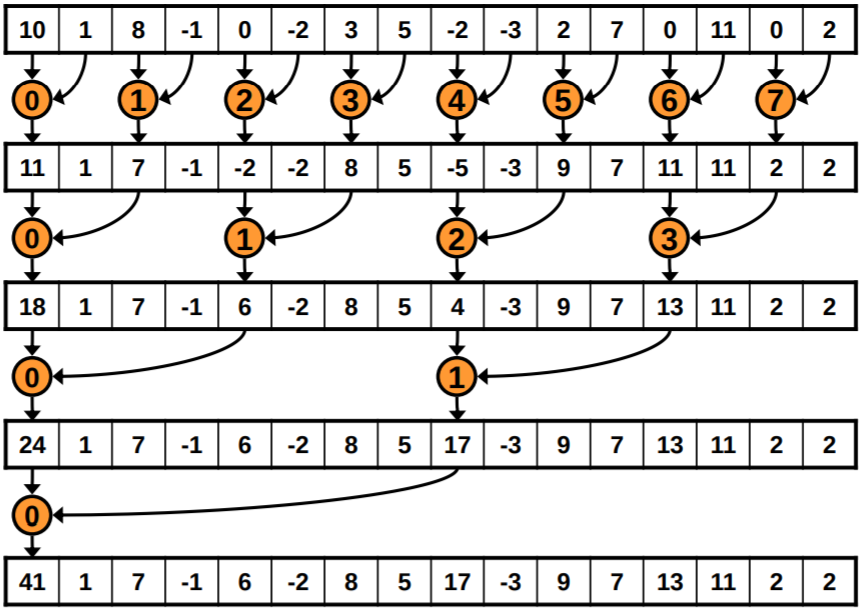
\includegraphics[width=0.5\linewidth, frame]{figures/session_2_figures/reduction.png}
\caption{Reduction of 16 values, pairing neighbours: stride 1, 2, 4, 8.}
\end{figure}

11 versus 11b:
\begin{itemize}[nosep]
  \item 11: thread \texttt{t} does \texttt{a[t] += a[t + stride]}, stride 8, 4, 2, 1.
  \item 11b: thread \texttt{t} works on \texttt{i = 2 * stride * t}, stride 1, 2, 4, 8.
\end{itemize}
Same result, same number of steps. In practice 11 is preferred: its active threads work on elements that sit next to each other (\texttt{a[0..stride-1]}), while in 11b the elements in use are \texttt{2 * stride} apart.
Elements next to each other are faster to access (see the Memory session).

\begin{lstlisting}[language=CUDA]
// description: the reduction of 11, pairing neighbours first, with the input of the figure. Print the whole array after every step.

#include <cstdio>

#define N 16

__global__ void reduce(int* a, int n) {
    int t = threadIdx.x;
    for (int stride = 1; stride < n; stride *= 2) {
        int i = 2 * stride * t;
        if (i < n) a[i] += a[i + stride];
        __syncthreads();

        // %3d: print the integer at least 3 characters wide, so the columns line up
        if (t == 0) {
            printf("stride %d:", stride);
            for (int k = 0; k < n; k++) printf(" %3d", a[k]);
            printf("\n");
        }
        __syncthreads();
    }
}

int main() {
    int input[N] = {10, 1, 8, -1, 0, -2, 3, 5, -2, -3, 2, 7, 0, 11, 0, 2};

    int* a;
    cudaMallocManaged(&a, N * sizeof(int));

    int expected = 0;
    printf("input:   ");
    for (int i = 0; i < N; i++) {
        a[i] = input[i];
        expected += input[i];
        printf(" %3d", a[i]);
    }
    printf("\n");

    reduce<<<1, N / 2>>>(a, N);
    cudaDeviceSynchronize();

    printf("sum = %d (expected %d)\n", a[0], expected);

    cudaFree(a);
}

// Output (compare with the figure, row by row):
// input:     10   1   8  -1   0  -2   3   5  -2  -3   2   7   0  11   0   2
// stride 1:  11   1   7  -1  -2  -2   8   5  -5  -3   9   7  11  11   2   2
// stride 2:  18   1   7  -1   6  -2   8   5   4  -3   9   7  13  11   2   2
// stride 4:  24   1   7  -1   6  -2   8   5  17  -3   9   7  13  11   2   2
// stride 8:  41   1   7  -1   6  -2   8   5  17  -3   9   7  13  11   2   2
// sum = 41 (expected 41)
\end{lstlisting}

\subsection{12\_reduction\_blocks.cu}

A block has at most 1024 threads, each handling 2 elements, so one block can reduce at most 2048 elements.
\texttt{\_\_syncthreads()} cannot synchronize different blocks, so for a large array the blocks are combined in another way.
12 combines both fixes:
\begin{itemize}[nosep]
  \item every block reduces its own chunk of the array, in shared memory;
  \item thread 0 of each block adds the block's result to the total with one \texttt{atomicAdd}.
\end{itemize}
For 1,000,000 elements: 1954 atomic operations instead of 1,000,000.

\begin{lstlisting}[language=CUDA]
// description: sum 1,000,000 elements. Every block reduces 512 elements in shared memory; thread 0 of each block adds the block result to the total with atomicAdd.

#include <cstdio>

#define N 1000000
#define THREADS 256

__global__ void reduce(const int* a, int* total, int n) {
    // __shared__ memory:
    //   - small, very fast memory on the GPU chip itself, one piece per block
    //   - all threads of the block can read and write it; other blocks cannot see it
    //   - it exists only while the block runs
    // A reduction reads and writes the same values many times; in shared memory that is much faster than in global memory.
    __shared__ int s[2 * THREADS];
    int t = threadIdx.x;
    int start = blockIdx.x * 2 * blockDim.x;

    // Each block handles 2 * 256 = 512 elements: every thread copies 2 of them to shared memory.
    // (cond) ? x : y means: if cond is true use x, otherwise y. A one-line if/else.
    // Elements beyond the end of the array are filled with 0, which does not change a sum. (For a maximum you would fill with the smallest int, INT_MIN.)
    s[t] = (start + t < n) ? a[start + t] : 0;
    s[t + blockDim.x] = (start + t + blockDim.x < n) ? a[start + t + blockDim.x] : 0;
    __syncthreads();

    for (int stride = blockDim.x; stride > 0; stride /= 2) {
        if (t < stride) s[t] += s[t + stride];
        __syncthreads();
    }

    // one atomicAdd per block
    if (t == 0) atomicAdd(total, s[0]);
}

int main() {
    int *a, *total;
    cudaMallocManaged(&a, N * sizeof(int));
    cudaMallocManaged(&total, sizeof(int));

    for (int i = 0; i < N; i++) a[i] = 1;
    *total = 0;

    int blocks = (N + 2 * THREADS - 1) / (2 * THREADS);
    reduce<<<blocks, THREADS>>>(a, total, N);
    cudaDeviceSynchronize();

    printf("blocks %d, expected %d, got %d\n", blocks, N, *total);

    cudaFree(a);
    cudaFree(total);
}

// Output:
// blocks 1954, expected 1000000, got 1000000
\end{lstlisting}

%=====================================================================
\section{CPU versus GPU}
\label{sec:timing}

13 compares the GPU with the CPU. The GPU is timed with CUDA events, as in 09. The CPU is timed with \texttt{std::chrono}, a normal C++ timer.

\subsection{13\_timing.cu}
\begin{lstlisting}[language=CUDA]
// description: sum 1,000,000 elements on the CPU and on the GPU (atomicAdd). Time both.

#include <cstdio>
// <chrono>: the C++ time library
#include <chrono>

#define N 1000000

__global__ void sum(const int* a, int* total, int n) {
    int i = blockIdx.x * blockDim.x + threadIdx.x;
    if (i < n) atomicAdd(total, a[i]);
}

int main() {
    int *a, *total;
    cudaMallocManaged(&a, N * sizeof(int));
    cudaMallocManaged(&total, sizeof(int));

    for (int i = 0; i < N; i++) a[i] = 1;

    // steady_clock::now(): the current time. The difference of two time points, converted to milliseconds, is the CPU time.
    auto c0 = std::chrono::steady_clock::now();
    int cpu = 0;
    for (int i = 0; i < N; i++) cpu += a[i];
    auto c1 = std::chrono::steady_clock::now();
    double cpu_ms = std::chrono::duration<double, std::milli>(c1 - c0).count();

    int threads = 256;
    int blocks = (N + threads - 1) / threads;

    // warm-up and GPU timing: as in 09
    sum<<<blocks, threads>>>(a, total, N);
    cudaMemset(total, 0, sizeof(int));

    cudaEvent_t start, stop;
    cudaEventCreate(&start);
    cudaEventCreate(&stop);

    cudaEventRecord(start);
    sum<<<blocks, threads>>>(a, total, N);
    cudaEventRecord(stop);
    cudaEventSynchronize(stop);

    float gpu_ms;
    cudaEventElapsedTime(&gpu_ms, start, stop);

    printf("CPU: sum %d in %.3f ms\n", cpu, cpu_ms);
    printf("GPU: sum %d in %.3f ms\n", *total, gpu_ms);

    cudaEventDestroy(start);
    cudaEventDestroy(stop);
    cudaFree(a);
    cudaFree(total);
}

// Output (the times depend on the machine):
// CPU: sum 1000000 in 100 ms
// GPU: sum 1000000 in 10 ms
\end{lstlisting}

%=====================================================================
\section{Locks}
\label{sec:locks}

An atomic makes one operation indivisible. A lock makes a whole piece of code indivisible: only one thread at a time can be between lock and unlock. That piece of code is the \emph{critical section}.
The principle is called \emph{mutex} (mutual exclusion): while a thread runs the critical section, all other threads are shut out.

Two threads A and B reach the same lock:
\begin{itemize}[nosep]
  \item A arrives first and takes the lock, executes the critical section, releases the lock, and continues in parallel.
  \item B arrives second and waits in the lock's loop until A releases the lock. Then B takes the lock and executes the critical section.
\end{itemize}

A lock is built with \texttt{atomicCAS(int* address, int compare, int val)} (compare-and-swap), which does as one indivisible step:
\begin{enumerate}[nosep]
  \item read the value \texttt{old} at \texttt{address};
  \item \texttt{*address = (old == compare) ? val : old};
  \item return \texttt{old}.
\end{enumerate}
In words: ``if \texttt{*address} is still \texttt{compare}, replace it with \texttt{val}''. The return value tells whether it worked: \texttt{old == compare} means this thread replaced the value.

The lock itself is one \texttt{int} in global memory, the mutex: 0 = free, 1 = taken.
\begin{itemize}[nosep]
  \item lock: \texttt{while (atomicCAS(mutex, 0, 1) != 0);} keeps trying until this thread changes 0 into 1;
  \item unlock: \texttt{atomicExch(mutex, 0);} sets it back to 0.
\end{itemize}

\subsection{14\_lock.cu}
\begin{lstlisting}[language=CUDA]
// description: thread 0 of every block adds 1 to a counter, once without and once with a lock. The correct result is the number of blocks.

#include <cstdio>

#define BLOCKS 512

// Race condition: thread 0 of all blocks does read + add + write on the same int.
__global__ void count(int* n) {
    if (threadIdx.x == 0) *n = *n + 1;
}

__global__ void count_locked(int* n, int* mutex) {
    if (threadIdx.x == 0) {
        // lock: atomicCAS returns the old value. 0 means this thread took the lock; otherwise it tries again (spinning).
        while (atomicCAS(mutex, 0, 1) != 0);
        // __threadfence(): makes sure this thread sees the writes of the previous owner of the lock
        __threadfence();

        // critical section: executed by one thread at a time
        *n = *n + 1;

        // __threadfence(): makes the write to n visible to the other threads before the lock is released
        __threadfence();
        // unlock
        atomicExch(mutex, 0);
    }
}

int main() {
    int *n, *mutex;
    cudaMallocManaged(&n, sizeof(int));
    cudaMallocManaged(&mutex, sizeof(int));

    *n = 0;
    count<<<BLOCKS, 256>>>(n);
    cudaDeviceSynchronize();
    printf("without lock: %d blocks\n", *n);

    *n = 0;
    *mutex = 0;
    count_locked<<<BLOCKS, 256>>>(n, mutex);
    cudaDeviceSynchronize();
    printf("with lock:    %d blocks\n", *n);

    cudaFree(n);
    cudaFree(mutex);
}

// Output (the first number is usually lower than 512 and changes from run to run):
// without lock: 233 blocks
// with lock:    512 blocks
//
// For one increment, atomicAdd(n, 1) is enough and faster. The lock is shown because it works for any amount of code in the critical section.
\end{lstlisting}

%=====================================================================
\section{Exercise: histogram (sessions 01 + 02)}
\label{sec:histogram}

An array of N values (for example N = 1,000,000), each from 0 to 9.
Count how many times each value occurs: a histogram with 10 bins.
Fill the array with any pattern you like, for example \texttt{a[i] = i \% 10}.

\begin{enumerate}[nosep]
  \item CPU version: loop over the array and do \texttt{hist[a[i]]++}. This is your reference.
  \item GPU version: one thread per element; every thread does \texttt{hist[a[i]]++}.
  \item Compare with the CPU:
    \begin{itemize}[nosep]
      \item Is every bin correct?
      \item Is the sum of all bins equal to N?
      \item Run it several times. Do you get the same result every time?
    \end{itemize}
  \item Explain what goes wrong. Which threads access the same memory location, and when?
  \item Fix it with \texttt{atomicAdd} and verify again.
\end{enumerate}

Questions:
\begin{itemize}[nosep]
  \item Why did the flip from session 01 have no race condition, while the histogram does?
  \item Would the race also happen if you launched only one thread?
\end{itemize}

\subsection{15\_histogram.cu (solution)}
\begin{lstlisting}[language=CUDA]
// description: solution. One program, two kernels, so the race condition is visible side by side:
//   hist_race: every thread does hist[a[i]]++               -> race condition, counts are too low
//   hist_ok:   every thread does atomicAdd(&hist[a[i]], 1)  -> correct
// a[i] = i % 10, so every bin must end up at N / 10 = 100000, and all bins together at N.

#include <cstdio>

#define N 1000000
#define BINS 10

__global__ void hist_race(const int* a, int* hist, int n) {
    int i = blockIdx.x * blockDim.x + threadIdx.x;
    if (i < n) hist[a[i]]++;
}

__global__ void hist_ok(const int* a, int* hist, int n) {
    int i = blockIdx.x * blockDim.x + threadIdx.x;
    if (i < n) atomicAdd(&hist[a[i]], 1);
}

int main() {
    int *a, *race, *ok;
    cudaMallocManaged(&a, N * sizeof(int));
    cudaMallocManaged(&race, BINS * sizeof(int));
    cudaMallocManaged(&ok, BINS * sizeof(int));
    int cpu[BINS] = {0};

    for (int i = 0; i < N; i++) a[i] = i % BINS;
    for (int i = 0; i < N; i++) cpu[a[i]]++;

    for (int b = 0; b < BINS; b++) {
        race[b] = 0;
        ok[b] = 0;
    }

    int threads = 256;
    int blocks = (N + threads - 1) / threads;
    hist_race<<<blocks, threads>>>(a, race, N);
    hist_ok<<<blocks, threads>>>(a, ok, N);
    cudaDeviceSynchronize();

    int sum_race = 0, sum_ok = 0;
    printf("bin      cpu     race       ok\n");
    for (int b = 0; b < BINS; b++) {
        printf("%3d %8d %8d %8d\n", b, cpu[b], race[b], ok[b]);
        sum_race += race[b];
        sum_ok += ok[b];
    }
    printf("sum %8d %8d %8d\n", N, sum_race, sum_ok);

    cudaFree(a);
    cudaFree(race);
    cudaFree(ok);
}

// Output (the "race" column is lower and changes from run to run):
// bin      cpu     race       ok
//   0   100000      ...   100000
//   1   100000      ...   100000
//   ...
//   9   100000      ...   100000
// sum  1000000      ...  1000000
//
// Why it races: there are only 10 bins, so many threads update the same bin at the same time.
// In every warp of 32 threads, 3 or 4 threads have the same value. Each ++ is read + add + write:
// threads read the same old count, both add 1, both write back -> increments are lost.
//
// Why the flip from session 01 had no race: there every thread wrote to its OWN output position,
// computed from its thread index. Here the write position depends on the DATA (the value a[i]),
// so different threads can end up writing to the same place.
//
// One thread: no race. A single thread does all increments one after another.
\end{lstlisting}

%=====================================================================
\section{Submission: maximum intensity projection}
\label{sec:submission}

In angiography, a contrast agent makes the blood vessels the brightest structures in a 3D scan.
A maximum intensity projection (MIP) shows them in one 2D image: every pixel $(x, y)$ gets the brightest voxel along $z$:
\[
  \mathit{mip}(x, y) = \max_{z} \; \mathit{vol}(x, y, z)
\]
This is max detection, once for every pixel: many voxels, one result per pixel.

\begin{figure}[H]
\centering
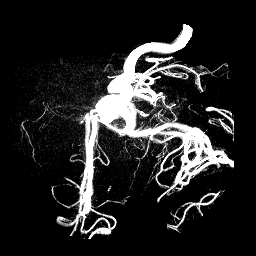
\includegraphics[width=0.4\linewidth, frame]{figures/session_2_figures/mip.png}
\caption{Expected result: the MIP of the aneurism volume (256 slices).}
\end{figure}

\subsection{Data}

The volume ``aneurism'' from the Open SciVis Datasets (\url{http://klacansky.com/open-scivis-datasets/}): a rotational C-arm X-ray scan of the arteries of the right half of a human head. A contrast agent was injected into the blood, and an aneurism is present.
\begin{itemize}[nosep]
  \item 256 $\times$ 256 $\times$ 256 voxels, one byte (\texttt{uint8}) per voxel, stored as raw bytes;
  \item order: $x$ fastest, then $y$, then $z$: voxel $(x, y, z)$ is at index \texttt{x + W * (y + H * z)}.
\end{itemize}

\texttt{volume.h} reads the volume and writes the result as a PGM image, which opens in a normal image viewer. The voxels are returned as \texttt{int} in managed memory, so they can be used directly in kernels and with \texttt{atomicMax}.

\begin{lstlisting}[language=CUDA]
// volume.h: read a raw 8-bit volume and write an 8-bit grayscale PGM image.
//
//   int* vol = read_volume("aneurism_256x256x256_uint8.raw", 256, 256, 256);  // w * h * d voxels: x fastest, then y, then z; values 0..255; managed memory
//   write_pgm("mip.pgm", mip, 256, 256);                     // values are clamped to 0..255
//   write_pgm("slice.pgm", vol + 128 * 256 * 256, 256, 256); // one slice (z = 128)
//   cudaFree(vol);
//
// With d smaller than the number of slices in the file, only the first d slices are read.

#pragma once
#include <cstdio>
#include <vector>

inline int* read_volume(const char* path, int w, int h, int d) {
    FILE* f = fopen(path, "rb");
    if (!f) {
        printf("cannot open %s\n", path);
        return nullptr;
    }
    size_t n = (size_t)w * h * d;
    std::vector<unsigned char> buf(n);
    size_t got = fread(buf.data(), 1, n, f);
    fclose(f);
    if (got != n) {
        printf("%s: expected %zu bytes, read %zu\n", path, n, got);
        return nullptr;
    }
    int* vol;
    cudaMallocManaged(&vol, n * sizeof(int));
    for (size_t i = 0; i < n; i++) vol[i] = buf[i];
    return vol;
}

inline void write_pgm(const char* path, const int* img, int w, int h) {
    FILE* f = fopen(path, "wb");
    if (!f) {
        printf("cannot open %s\n", path);
        return;
    }
    fprintf(f, "P5\n%d %d\n255\n", w, h);
    for (int i = 0; i < w * h; i++) {
        int v = img[i] < 0 ? 0 : (img[i] > 255 ? 255 : img[i]);
        fputc(v, f);
    }
    fclose(f);
}
\end{lstlisting}

\subsection{How to use volume.h}
\begin{enumerate}[nosep]
  \item Download the volume into the same folder as your \texttt{.cu} file and \texttt{volume.h}. The file must be 16,777,216 bytes ($256^3$):\\
    \texttt{wget} \url{http://klacansky.com/open-scivis-datasets/aneurism/aneurism_256x256x256_uint8.raw}
  \item Include \texttt{volume.h} and use it as below.
  \item Compile and run: \texttt{nvcc -o mip mip.cu}, then \texttt{./mip}. Open \texttt{mip.pgm} and \texttt{slice.pgm} in an image viewer.
  \item For the timing, change \texttt{D} to 16, 32, 64 or 128: only the first \texttt{D} slices are read.
\end{enumerate}

\begin{lstlisting}[language=CUDA]
#include <cstdio>
#include "volume.h"

#define W 256
#define H 256
#define D 256

int main() {
    // read the first D slices; returns nullptr if the file is missing or too short
    int* vol = read_volume("aneurism_256x256x256_uint8.raw", W, H, D);
    if (!vol) return 1;

    int* mip;
    cudaMallocManaged(&mip, W * H * sizeof(int));

    // ... compute the MIP here ...
    // voxel (x, y, z): vol[x + W * (y + H * z)]
    // pixel (x, y):    mip[x + W * y]

    write_pgm("mip.pgm", mip, W, H);

    // vol + z * W * H points to slice z: here the middle slice
    write_pgm("slice.pgm", vol + (D / 2) * W * H, W, H);

    cudaFree(vol);
    cudaFree(mip);
}
\end{lstlisting}

\subsection{Tasks}
\begin{enumerate}[nosep]
  \item CPU: compute the MIP with a loop over $x$, $y$ and $z$, and write it as an image. This is your reference.
  \item GPU, race: one thread per voxel (a 3D grid of 3D blocks, for example 8 $\times$ 8 $\times$ 8 threads). Every thread does \texttt{if (v > mip[p]) mip[p] = v;}.
  \item GPU, atomics: the same kernel with \texttt{atomicMax(\&mip[p], v)}.
  \item GPU, reduction: one block per pixel. The threads of the block find the maximum of the voxels in that column with a reduction in shared memory; thread 0 writes it to \texttt{mip}.
  \item GPU, one thread per column: one thread per pixel, which loops over all $z$.
  \item Correctness: count the pixels that differ from the CPU result, for every GPU version.
  \item Timing: time the CPU, atomics, reduction and one-thread-per-column versions for $d$ = 16, 32, 64, 128 and 256 slices (read only the first $d$ slices). Plot the time as a function of the number of voxels.
\end{enumerate}

Timing rules:
\begin{itemize}[nosep]
  \item GPU: CUDA events around the kernel launch only. No allocation, no copies and no file reading or writing between the events.
  \item No CPU access to \texttt{vol} or \texttt{mip} between the warm-up and the end of the timed runs: a CPU access moves the managed memory back to the CPU, and the next kernel has to move it back first.
  \item Set \texttt{mip} to 0 once, before the warm-up launch. It needs no reset between the runs: the same volume gives the same maximum.
  \item CPU: \texttt{std::chrono} around the loops only.
  \item Do one warm-up launch before timing (as in 09).
  \item Report the average of 10 runs.
  \item Plot with logarithmic axes for both the time and the number of voxels.
\end{itemize}

\subsection{Questions}
\begin{itemize}[nosep]
  \item How does the execution time grow with the number of voxels? Where does the GPU overtake the CPU, and why is the GPU slower for small volumes?
  \item How many pixels does the race version get wrong? Why not all of them?
  \item The one-thread-per-column version uses far fewer threads. Does it need \texttt{atomicMax}? Which version is fastest, and why?
  \item Your reduction uses one block per pixel. What would you change if a column had more than 2048 voxels?
\end{itemize}

\subsection{Report}
Hand in a one-page report with:
\begin{itemize}[nosep]
  \item slice $z = 128$ and the MIP, side by side;
  \item the correctness table;
  \item the timing plot;
  \item the answers to the questions.
\end{itemize}

%=====================================================================
\section{Lexicon}
\label{sec:lexicon}

\begin{description}[nosep]
  \item[ALU] Arithmetic logic unit: the part of a GPU core that does the integer arithmetic.
  \item[Atomic operation] Read + modify + write as one indivisible step. Atomics on the same address are executed one after another.
  \item[\texttt{atomicCAS}] Compare-and-swap: if \texttt{*address} equals \texttt{compare}, replace it with \texttt{val}. Returns the old value.
  \item[Contrast stretching] Mapping the pixel values of an image so that the darkest pixel becomes 0 and the brightest 255.
  \item[Critical section] The code between lock and unlock, executed by one thread at a time.
  \item[CUDA event] A timestamp recorded by the GPU, in order with the kernels. Used to time GPU work.
  \item[Global memory] The large GPU memory (DRAM), visible to all threads of all blocks.
  \item[L2 cache] Cache shared by all SMs, between the SMs and global memory. Atomics on global memory are executed here.
  \item[Lock] A mechanism that lets only one thread at a time execute a piece of code.
  \item[Managed memory] Memory allocated with \texttt{cudaMallocManaged}, usable from the CPU and the GPU.
  \item[Memory fence] \texttt{\_\_threadfence()}: the writes of a thread before the fence become visible to other threads before its writes after the fence.
  \item[Mutex] Mutual exclusion: the principle behind locks. Also the variable that holds the state of a lock.
  \item[PGM] A simple image file format: a short text header followed by one byte per pixel.
  \item[Race condition] The result of a program depends on the timing of events that cannot be controlled, such as the execution order of threads.
  \item[Reduction] Combining many values into one (sum, maximum, \ldots) by combining pairs in parallel: $N$ values take $\log_2 N$ steps.
  \item[Register] The fastest storage on the GPU, private to one thread.
  \item[Shared memory] Small, fast memory on the GPU chip, one piece per block, visible to all threads of that block. It exists only while the block runs.
  \item[SM] Streaming multiprocessor: a GPU core that executes blocks.
  \item[Spinning] A thread retrying in a loop until a lock is free.
  \item[Stride] In a reduction: the distance between the two elements that are added.
  \item[\texttt{\_\_syncthreads()}] Barrier: all threads of a block wait until every thread of that block has arrived.
  \item[Warm-up] A first kernel launch before timing, so one-time costs are not measured.
  \item[Warp] 32 threads that execute the same instruction together.
\end{description}

\end{document}
